%\part{Entwurfsprinzipien}

%----------------------------------------------------------------------------
\section{Requirements Engineering}
\begin{frame}[fragile]
	\frametitle{Requirements Engineering}
\huge Requirements Engineering
\end{frame}

\begin{frame}
\frametitle{Requirements Engineering}
	\begin{itemize}
		\item Anforderungen des Kunden an die Software sind der zentrale Faktor in einem Softwareprojekt!
		\item Wenn die Anforderungen des Kunden nicht erfüllt werden ist die Software wertlos
		\item Die systematische Ermittlung, Analyse und Spezifikation der Anforderungen wird als Systemanalyse
					oder Requirements Engineering bezeichnet
	\end{itemize}
	\begin{block}{Anforderung}
		Anforderungen (requirements) legen fest, was von einem Softwaresystem als Eigenschaft erwartet wird.
  \end{block}
\end{frame}

\begin{frame}
\frametitle{6 Dimensionen der Komplexität}
	Komplexität der Funktionen
	\begin{itemize}
		\item Software wird komplexer je mehr Funktionen sie besitzt
		\item Beispiel: Integrierte Büroanwendungen
		\begin{itemize}
			\item Tabellenkalkulation, Präsentationen, Textverarbeitung, Datenbank
			\item 1000 - 1500 Funktionen
		\end{itemize}
	\end{itemize}
	\bigskip
	Komplexität der Daten
	\begin{itemize}
		\item Wird durch Vielzahl von Datenstrukturen oder sehr komplexen Datenstrukturen definiert
		\item Beispiel: DB-orientierte Systeme, Datawarehouses, Big Data Applikationen
	\end{itemize}
\end{frame}

\begin{frame}
\frametitle{6 Dimensionen der Komplexität}
	Komplexität der Algorithmen
	\begin{itemize}
		\item Systeme die komplexe numerische Berechnungen durchführen
	\end{itemize}
	\bigskip
	Komplexität des zeitabhängigen Verhaltens
	\begin{itemize}
		\item Wird durch viele nebenläufige Prozesse, gegenseitiges Ausschließen oder Zeitbedingungen gekennzeichnet
		\item Beispiele sind Betriebssysteme, Prozesssteuerungen, verteilte Systeme
	\end{itemize}
\end{frame}

\begin{frame}
\frametitle{6 Dimensionen der Komplexität}
	Komplexität der Systemumgebung
	\begin{itemize}
		\item Systeme bei denen es im wesentlichen auf das Zusammenwirken mit dem Gesamtsystem ankommt
		\item Beispiel: Embedded Systems (Flugzeugsteuerungen, Fahrzeugsysteme), IOT Lösungen
	\end{itemize}
	\bigskip
	Komplexität der Benutzeroberfläche
	\begin{itemize}
		\item Systeme mit komplexer Interaktion zwischen Anwender und Computersystem
		\item Beispiel: CAD-Systeme, CASE-Syteme, Büro- und Enterpriseanwendungen
	\end{itemize}
\end{frame}

\begin{frame}
\frametitle{6 Dimensionen der Komplexität}
	Das Modellierungskonzept ist entsprechend der Komplexität des zu entwickelnden Produkts auszuwählen.
	Weist das zugrundeliegende Produkt beispielsweise eine hohe Komplexität der Funktionen auf, so muss das verwendete
	Konzept es erlauben eine Vielzahl von Funktionen zu modellieren.
\end{frame}

\begin{frame}
\frametitle{Analyse und Entwurf mit UML}
	\begin{columns}
			\begin{column}{.5\textwidth}
			\small
			\begin{itemize}
				\item Unified Modeling Language
				\item Sprache zur objektorientierten Modellierung
				\item Standardisiert von der OMG
				\item Auch zur Implementierung genutzt
			\end{itemize}
			\normalsize
			\end{column}
			\begin{column}{.5\textwidth}
				\center
				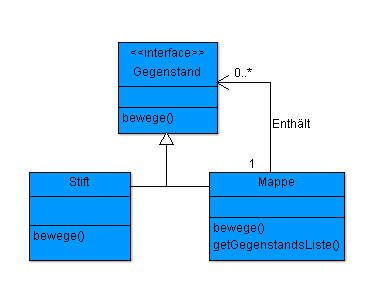
\includegraphics[width=1\textwidth,
				keepaspectratio=true]{bilder/uml_example.png}
			\end{column}
	\end{columns}
\end{frame}

\begin{frame}
\frametitle{Analyse und Entwurf mit UML}
		Berücksichtigung aktueller Trends der Softwareentwicklung
		\begin{itemize}
			\item Patterns
			\item Komponentenorientiertes Design
			\item Anwendungsfälle modellieren
			\item Ausführbarkeit von Modellen
		\end{itemize}
\end{frame}

\begin{frame}
\frametitle{Analyse und Entwurf mit UML}
	OOA (Objektorientierte Analyse) = Anwendersicht
	\begin{itemize}
		\item Modell der Anforderungen
	\end{itemize}
	\bigskip
	OOD (Objektorientiertes Design) = Entwicklersicht
	\begin{itemize}
	 \item Details und Randbedingungen
	\end{itemize}
  \bigskip
	OOP (Objektorientierte Progr.) = Entwicklersicht
	\begin{itemize}
		\item Implementierung
	\end{itemize}
\end{frame}

\begin{frame}
\frametitle{Exkurs OOP: Objekte, Methoden und Attribute}
	\center
	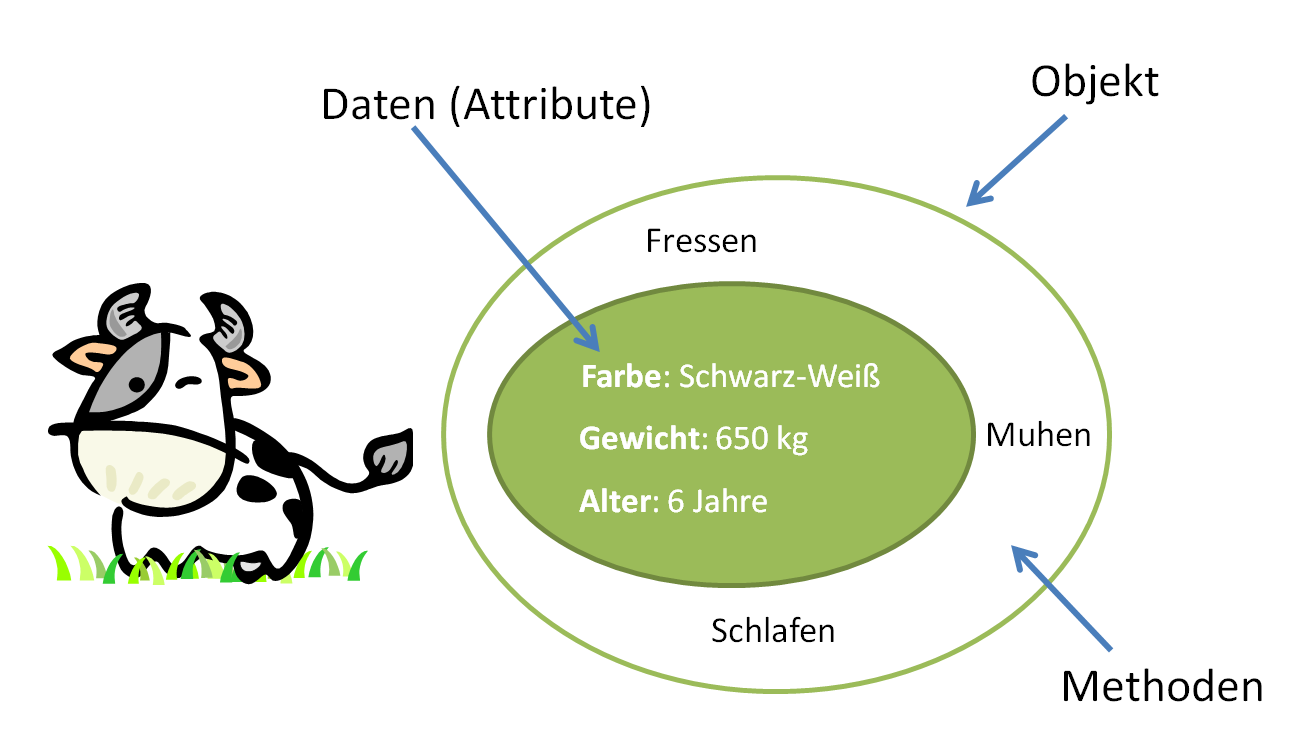
\includegraphics[width=0.9\textwidth, keepaspectratio=true]{bilder/kuh.png}
\end{frame}

\begin{frame}
\frametitle{Exkurs OOP: Klassen als Objektbauplan}
	\begin{columns}
	    \begin{column}{.6\textwidth}
			\small
			\begin{itemize}
			  \item Klasse fungiert als Bauplan f\"ur Objekte
			  \item Aus diesem Bauplan lassen sich beliebig viele Objekte erzeugen
			  \item Objekte aus einer Klasse besitzen die gleichen Methoden
			  \item Objekte aus einer Klasse besitzen die gleichen Attribute \\(Werte
			  k\"onnen jedoch variieren)
			  \item Klassen k\"onnen durch Vererbung weiter spezialisiert werden
			\end{itemize}
			\normalsize
	    \end{column}
	    \begin{column}{.4\textwidth}
	   		\center
			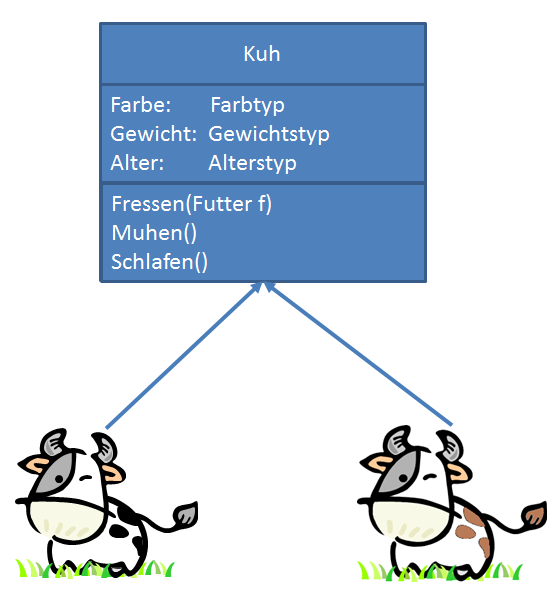
\includegraphics[width=\textwidth,
			keepaspectratio=true]{bilder/kuh_klasse.png}
	    \end{column}
	\end{columns}
\end{frame}

\begin{frame}
\frametitle{Exkurs OOP: Beziehungen zwischen Objekten}
\begin{columns}
	    \begin{column}{.6\textwidth}
			\small
			\begin{itemize}
			  \item Zwischen Objekten k\"onnen Beziehungen existieren
			  \begin{item}
			  		Beziehung zwischen Bauer und Kuh:
					\begin{enumerate}
					  \item \tiny Der Bauer kann 0 bis n K\"uhe besitzen
					  \item \tiny Eine Kuh geh\"ort genau einem Bauer
					  \item \tiny Keine Kuh kann einen Bauer besitzen \\ (gerichtete Beziehung)
					\end{enumerate}
			  \end{item}
			\end{itemize}
			\normalsize
	    \end{column}
	    \begin{column}{.4\textwidth}
	   		\center
			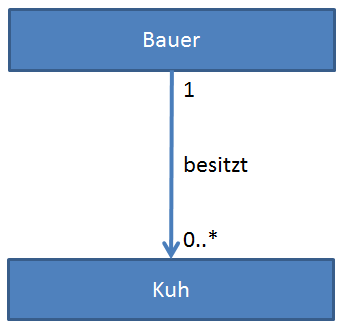
\includegraphics[width=0.9\textwidth,
			keepaspectratio=true]{bilder/asso_kuh.png}
	    \end{column}
	\end{columns}
\end{frame}

\begin{frame}
\frametitle{Exkurs OOP: Methodenaufrufe}
\begin{columns}
	    \begin{column}{.6\textwidth}
			\small
			\begin{itemize}
			  \item Objekte k\"onnen sich untereinander Botschaften senden
			  \item Damit wird der Empf\"anger aufgefordert etwas auszuf\"uhren
			  \begin{item}
			  		Erweitern wir die Klasse ''Kuh''
					\begin{enumerate}
					  \item \tiny Kuh bekommt die Methode: ''gebeMilch''
					  \item \tiny ''gebeMilch'' gibt ein Objekt vom Typ ''Milchtyp'' zur\"uck
					\end{enumerate}
			  \end{item}
			  \item Der Bauer l\"ost durch senden einer Botschaft die Methode
			  ''gebeMilch'' aus
			  \item Die Kuh f\"uhrt die Methode aus und gibt Milchtyp-Objekt zur\"uck
			\end{itemize}
			\normalsize
	    \end{column}
	    \begin{column}{.4\textwidth}
	   		\center
			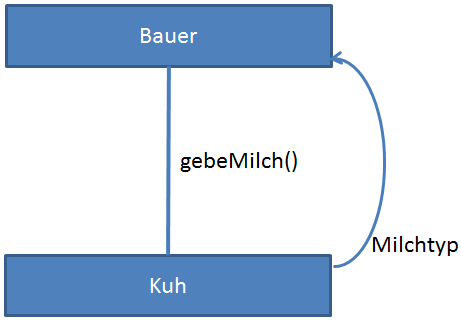
\includegraphics[width=1\textwidth,
			keepaspectratio=true]{bilder/methodenaufruf.png}
	    \end{column}
	\end{columns}
\end{frame}

\subsection{Use Cases}
\begin{frame}
\frametitle{Use Cases}
	\begin{block}{Use Case}
		Ein Use Case beschreibt Szenarien einzelner Interaktionen zwischen dem Nutzer und dem System.
	\end{block}
	\bigskip
	Zielsetzung
	\begin{itemize}
		\item Spezifikation der Funktionalität des Systems
		\item Identifikation: Wer / was arbeitet mit dem System
		\item Trennung zwischen dem was das System leistet und was außerhalb bearbeitet wird
		\item Zergliederung in Einheiten mit Akteuren und den zugehörigen Anwendungsfällen
	\end{itemize}
\end{frame}

\begin{frame}
\frametitle{Use Case Beispiel}
	\center
	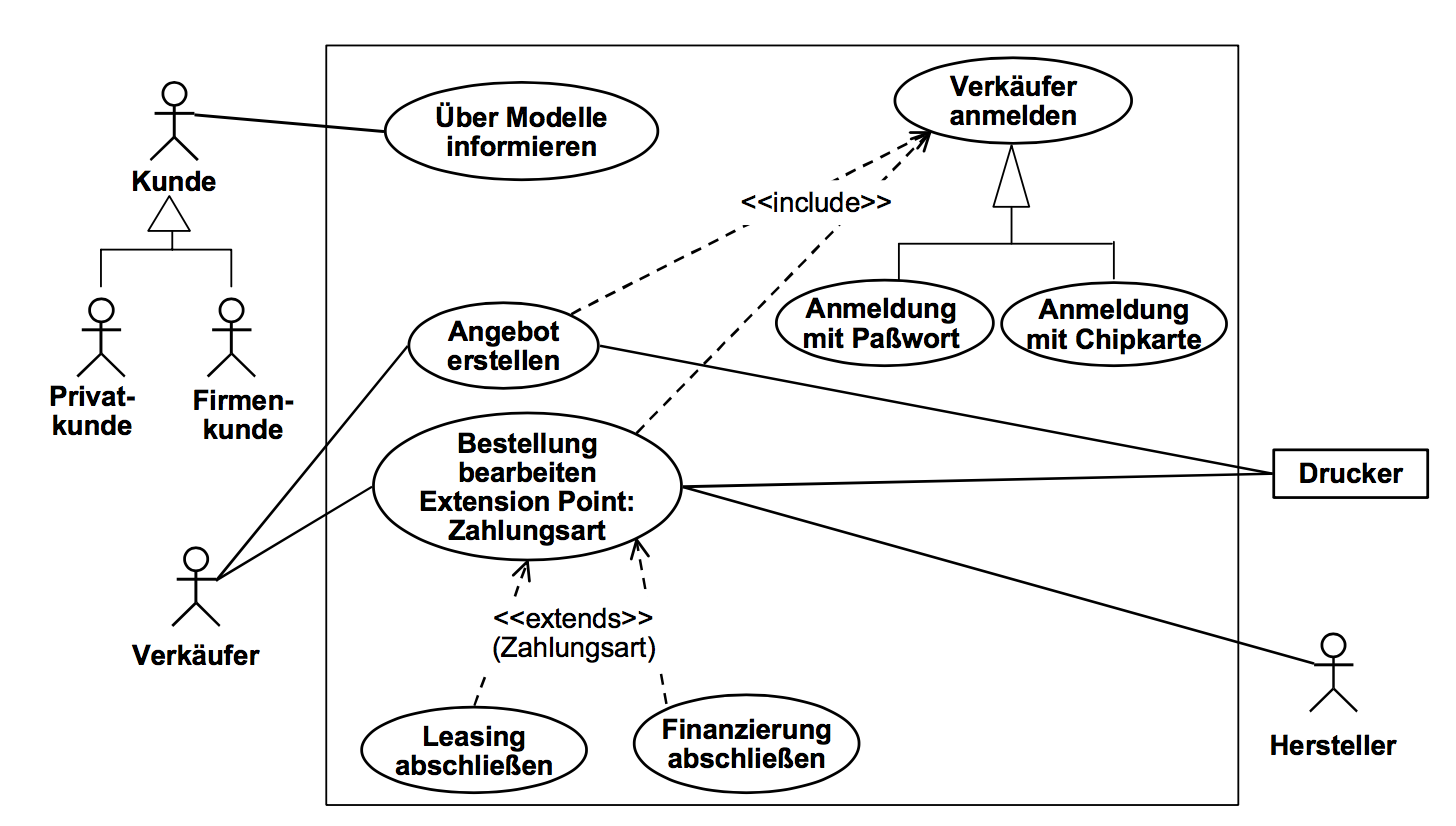
\includegraphics[width=1\textwidth,
	keepaspectratio=true]{bilder/use_case_beispiel.png}
\end{frame}

\begin{frame}
\frametitle{Use Cases}
	Beschreiben die Interaktionen zwischen den Akteuren und dem System
	\begin{itemize}
		\item Wie wird das System verwendet?
		\item Welches Verhalten zeigt das System nach außen?
		\item Use Cases werden stets von einem Akteur angestoßen,
					um bestimmte Funktionalität des Systems zu nutzen
	\end{itemize}
\end{frame}

\begin{frame}
\frametitle{Use Cases}
	Beschreiben alle Abläufe die zur Durchführung nötig sind
	\begin{itemize}
		\item Nur Abläufe und Schritte die nach außen sichtbar sind
		\item Keine internen Strukturen
	\end{itemize}
\end{frame}

\begin{frame}
\frametitle{Use Cases}
	Sind in sich abgeschlossen
	\begin{itemize}
		\item Alle Abläufe sind vollständig enthalten
		\item Jeder Use Case kann für sich allein bestehen und ist für sich allein sinnvoll
		\item Jeder Use Case liefert ein Resultat für mindestens einen Akteur
	\end{itemize}
	\bigskip
	Alle Use Cases modellieren in ihrer Gesamtheit das funktionale Verhalten des Systems
\end{frame}
